%!TEX root = ../main.tex

To sum up, \textit{PEM identification} is a common paradigm for finding suitable models from data, based on prediction theory.

We have to move from stochastic models (ARMAX models) of type: 

$$
M(\theta):
y(t) \ =\ \frac{B(z,\theta)}{A(z,\theta)} u(t-d) \ +\ \frac{C(z,\theta)}{A(z,\theta)} e(t) ,\ e(t)\sim \WN \left(0,\lambda ^{2}\right)
$$

to models in prediction form, i.e. the optimal predictors obtained through the theory we developed. In particular, we can focus on the one-step predictor already introduced:

$$
\hat{M}(\theta) :
\ \hat{y}(t\mid t-1) \ =\frac{B(z,\theta) E(z,\theta) \ }{C(z,\theta)} u(t-d) \ +\ \frac{F(z,\theta)}{C(z,\theta)} y(t-1)
$$

The predictor has a different structure: while $ M(\theta)$ is fed by \gls{wn} and input $u$, the predictor $\hat{M}(\theta)$ is fed by measurements of $u$ and $y$ and returns the predicted future values of output, \textbf{there isn't \gls{wn}}. The predictor model is returning the predicted values for \textit{that} realization of input and output.


\tikzset{every picture/.style={line width=0.75pt}} %set default line width to 0.75pt        

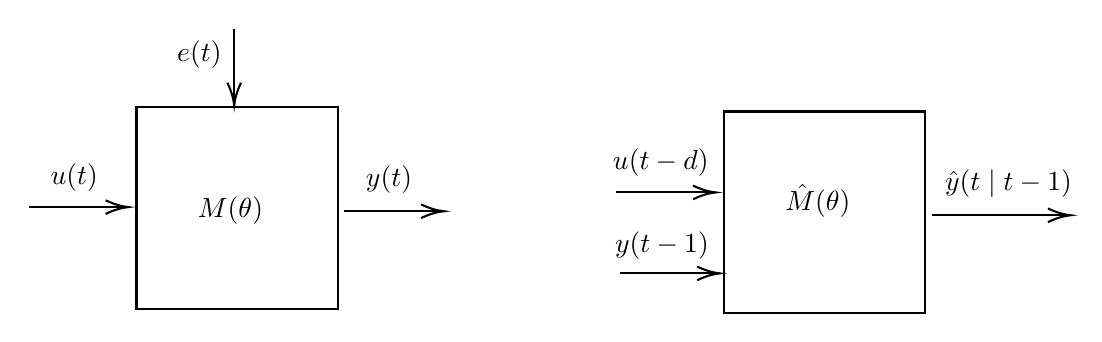
\begin{tikzpicture}[x=0.75pt,y=0.75pt,yscale=-1,xscale=1]
%uncomment if require: \path (0,173); %set diagram left start at 0, and has height of 173

%Shape: Square [id:dp2606700449895307] 
\draw   (66.94,52) -- (164,52) -- (164,149.06) -- (66.94,149.06) -- cycle ;
%Straight Lines [id:da7364516735552062] 
\draw    (114,14.06) -- (114,49) ;
\draw [shift={(114,51)}, rotate = 270] [color={rgb, 255:red, 0; green, 0; blue, 0 }  ][line width=0.75]    (10.93,-3.29) .. controls (6.95,-1.4) and (3.31,-0.3) .. (0,0) .. controls (3.31,0.3) and (6.95,1.4) .. (10.93,3.29)   ;
%Straight Lines [id:da3618183623060065] 
\draw    (15,100) -- (61,100) ;
\draw [shift={(63,100)}, rotate = 180] [color={rgb, 255:red, 0; green, 0; blue, 0 }  ][line width=0.75]    (10.93,-3.29) .. controls (6.95,-1.4) and (3.31,-0.3) .. (0,0) .. controls (3.31,0.3) and (6.95,1.4) .. (10.93,3.29)   ;
%Straight Lines [id:da40706010732580533] 
\draw    (167,102) -- (213,102) ;
\draw [shift={(215,102)}, rotate = 180] [color={rgb, 255:red, 0; green, 0; blue, 0 }  ][line width=0.75]    (10.93,-3.29) .. controls (6.95,-1.4) and (3.31,-0.3) .. (0,0) .. controls (3.31,0.3) and (6.95,1.4) .. (10.93,3.29)   ;
%Shape: Square [id:dp23583643845840108] 
\draw   (349.94,53.94) -- (447,53.94) -- (447,151) -- (349.94,151) -- cycle ;
%Straight Lines [id:da7226691724323739] 
\draw    (298,92.94) -- (344,92.94) ;
\draw [shift={(346,92.94)}, rotate = 180] [color={rgb, 255:red, 0; green, 0; blue, 0 }  ][line width=0.75]    (10.93,-3.29) .. controls (6.95,-1.4) and (3.31,-0.3) .. (0,0) .. controls (3.31,0.3) and (6.95,1.4) .. (10.93,3.29)   ;
%Straight Lines [id:da7790245551294717] 
\draw    (450,103.94) -- (515,103.94) ;
\draw [shift={(517,103.94)}, rotate = 180] [color={rgb, 255:red, 0; green, 0; blue, 0 }  ][line width=0.75]    (10.93,-3.29) .. controls (6.95,-1.4) and (3.31,-0.3) .. (0,0) .. controls (3.31,0.3) and (6.95,1.4) .. (10.93,3.29)   ;
%Straight Lines [id:da18553981986249823] 
\draw    (300,131.94) -- (346,131.94) ;
\draw [shift={(348,131.94)}, rotate = 180] [color={rgb, 255:red, 0; green, 0; blue, 0 }  ][line width=0.75]    (10.93,-3.29) .. controls (6.95,-1.4) and (3.31,-0.3) .. (0,0) .. controls (3.31,0.3) and (6.95,1.4) .. (10.93,3.29)   ;

% Text Node
\draw (95,93.4) node [anchor=north west][inner sep=0.75pt]    {$M(\theta)$};
% Text Node
\draw (85,18.4) node [anchor=north west][inner sep=0.75pt]    {$e(t)$};
% Text Node
\draw (24,77.4) node [anchor=north west][inner sep=0.75pt]    {$u(t)$};
% Text Node
\draw (176,78.4) node [anchor=north west][inner sep=0.75pt]    {$y(t)$};
% Text Node
\draw (378,87.34) node [anchor=north west][inner sep=0.75pt]    {$\hat{M}(\theta)$};
% Text Node
\draw (295,70.34) node [anchor=north west][inner sep=0.75pt]    {$u(t-d)$};
% Text Node
\draw (455,80.34) node [anchor=north west][inner sep=0.75pt]    {$\hat{y}(t\mid t-1)$};
% Text Node
\draw (296,110.34) node [anchor=north west][inner sep=0.75pt]    {$y(t-1)$};


\end{tikzpicture}

The idea is that, when dealing with a real system, values of $u$ and $y$ from time $t=1,\ldots,n$ can be collected, subsequently taking the predictor (introducing proper delays $ z^{-1}$) and feeding it with the measurement of $u$ and $y$ collected during the experiment. Then, the output of the predictor $ \hat{M}(\theta $) can be used to construct the value of the \textbf{prediction error} $ \varepsilon $. 





\tikzset{every picture/.style={line width=0.75pt}} %set default line width to 0.75pt        

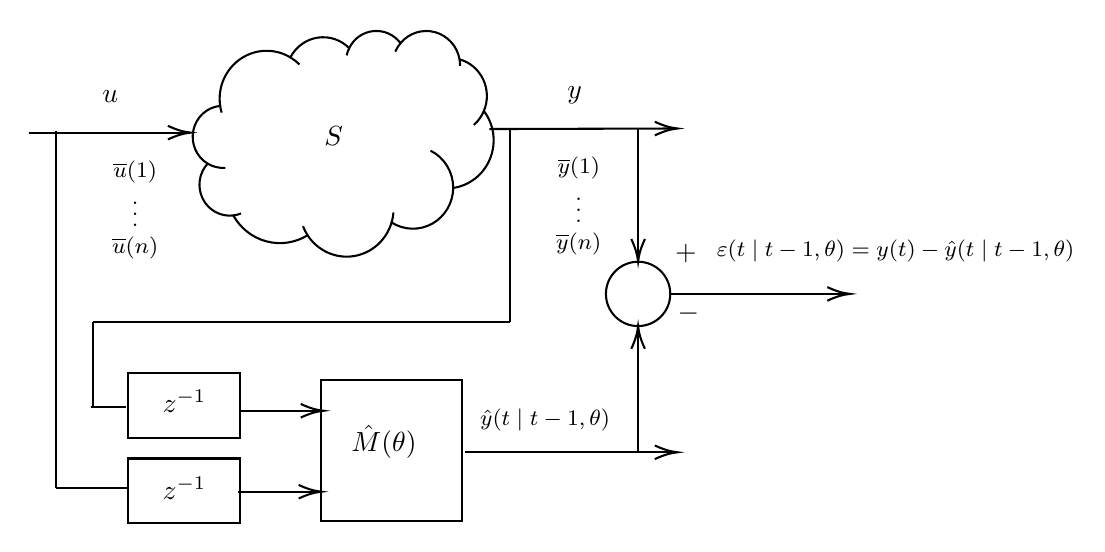
\begin{tikzpicture}[x=0.75pt,y=0.75pt,yscale=-1,xscale=1]
%uncomment if require: \path (0,300); %set diagram left start at 0, and has height of 300

%Shape: Cloud [id:dp9405713107767868] 
\draw   (111.2,74.8) .. controls (110.03,66.04) and (113.86,57.36) .. (121.07,52.45) .. controls (128.28,47.54) and (137.59,47.26) .. (145.07,51.74) .. controls (147.72,46.64) and (152.56,43.12) .. (158.14,42.24) .. controls (163.72,41.36) and (169.37,43.23) .. (173.4,47.28) .. controls (175.65,42.66) and (180.08,39.55) .. (185.11,39.07) .. controls (190.14,38.58) and (195.06,40.78) .. (198.12,44.89) .. controls (202.2,39.99) and (208.68,37.93) .. (214.77,39.59) .. controls (220.85,41.26) and (225.45,46.35) .. (226.57,52.68) .. controls (231.56,54.07) and (235.72,57.61) .. (237.97,62.38) .. controls (240.22,67.15) and (240.34,72.68) .. (238.3,77.55) .. controls (243.22,84.09) and (244.37,92.8) .. (241.32,100.43) .. controls (238.28,108.07) and (231.49,113.48) .. (223.5,114.65) .. controls (223.45,121.81) and (219.6,128.39) .. (213.45,131.84) .. controls (207.3,135.29) and (199.8,135.08) .. (193.84,131.28) .. controls (191.31,139.86) and (184.17,146.18) .. (175.51,147.5) .. controls (166.85,148.82) and (158.23,144.9) .. (153.36,137.45) .. controls (147.4,141.12) and (140.25,142.18) .. (133.52,140.38) .. controls (126.78,138.59) and (121.04,134.09) .. (117.58,127.9) .. controls (111.49,128.63) and (105.6,125.4) .. (102.83,119.82) .. controls (100.07,114.24) and (101.01,107.5) .. (105.21,102.93) .. controls (99.77,99.66) and (97,93.18) .. (98.33,86.85) .. controls (99.67,80.53) and (104.81,75.81) .. (111.07,75.14) ; \draw   (105.21,102.93) .. controls (107.77,104.48) and (110.73,105.18) .. (113.7,104.94)(117.58,127.9) .. controls (118.85,127.75) and (120.1,127.42) .. (121.3,126.94)(153.36,137.45) .. controls (152.47,136.07) and (151.72,134.6) .. (151.13,133.07)(193.84,131.28) .. controls (194.31,129.72) and (194.61,128.1) .. (194.74,126.47)(223.5,114.65) .. controls (223.56,107.02) and (219.32,100.03) .. (212.6,96.69)(238.3,77.55) .. controls (237.21,80.15) and (235.55,82.45) .. (233.45,84.28)(226.57,52.68) .. controls (226.75,53.73) and (226.84,54.79) .. (226.82,55.86)(198.12,44.89) .. controls (197.11,46.11) and (196.27,47.48) .. (195.64,48.94)(173.4,47.28) .. controls (172.86,48.39) and (172.45,49.57) .. (172.19,50.78)(145.07,51.74) .. controls (146.65,52.68) and (148.11,53.82) .. (149.42,55.13)(111.2,74.8) .. controls (111.36,76.01) and (111.61,77.21) .. (111.95,78.37) ;
%Straight Lines [id:da14261299446641984] 
\draw    (19,88) -- (95,88) ;
\draw [shift={(97,88)}, rotate = 180] [color={rgb, 255:red, 0; green, 0; blue, 0 }  ][line width=0.75]    (10.93,-3.29) .. controls (6.95,-1.4) and (3.31,-0.3) .. (0,0) .. controls (3.31,0.3) and (6.95,1.4) .. (10.93,3.29)   ;
%Straight Lines [id:da25912476814098584] 
\draw    (241,86.27) -- (329.6,86.01) ;
\draw [shift={(331.6,86)}, rotate = 179.83] [color={rgb, 255:red, 0; green, 0; blue, 0 }  ][line width=0.75]    (10.93,-3.29) .. controls (6.95,-1.4) and (3.31,-0.3) .. (0,0) .. controls (3.31,0.3) and (6.95,1.4) .. (10.93,3.29)   ;
%Straight Lines [id:da5081454591632601] 
\draw    (121,222) -- (159,222) ;
\draw [shift={(161,222)}, rotate = 180] [color={rgb, 255:red, 0; green, 0; blue, 0 }  ][line width=0.75]    (10.93,-3.29) .. controls (6.95,-1.4) and (3.31,-0.3) .. (0,0) .. controls (3.31,0.3) and (6.95,1.4) .. (10.93,3.29)   ;
%Straight Lines [id:da4200986918290637] 
\draw    (229,242) -- (329.6,242) ;
\draw [shift={(331.6,242)}, rotate = 180] [color={rgb, 255:red, 0; green, 0; blue, 0 }  ][line width=0.75]    (10.93,-3.29) .. controls (6.95,-1.4) and (3.31,-0.3) .. (0,0) .. controls (3.31,0.3) and (6.95,1.4) .. (10.93,3.29)   ;
%Straight Lines [id:da4094784213264089] 
\draw    (120,261) -- (158,261) ;
\draw [shift={(160,261)}, rotate = 180] [color={rgb, 255:red, 0; green, 0; blue, 0 }  ][line width=0.75]    (10.93,-3.29) .. controls (6.95,-1.4) and (3.31,-0.3) .. (0,0) .. controls (3.31,0.3) and (6.95,1.4) .. (10.93,3.29)   ;
%Shape: Square [id:dp8122731422115212] 
\draw   (159.94,207.06) -- (227.88,207.06) -- (227.88,275) -- (159.94,275) -- cycle ;
%Straight Lines [id:da908171537673635] 
\draw    (32,87) -- (32,259.2) ;
%Straight Lines [id:da8800162432572618] 
\draw    (49,220) -- (66,220) ;
%Straight Lines [id:da8482189437756391] 
\draw    (32,259.2) -- (67,259.2) ;
%Shape: Rectangle [id:dp380347788068776] 
\draw   (67,204) -- (121,204) -- (121,235.2) -- (67,235.2) -- cycle ;
%Shape: Rectangle [id:dp31523487953797846] 
\draw   (67,245) -- (121,245) -- (121,276.2) -- (67,276.2) -- cycle ;
%Straight Lines [id:da12922420940431545] 
\draw    (312.6,86.2) -- (312.6,148.2) ;
\draw [shift={(312.6,150.2)}, rotate = 270] [color={rgb, 255:red, 0; green, 0; blue, 0 }  ][line width=0.75]    (10.93,-3.29) .. controls (6.95,-1.4) and (3.31,-0.3) .. (0,0) .. controls (3.31,0.3) and (6.95,1.4) .. (10.93,3.29)   ;
%Straight Lines [id:da17484084938101363] 
\draw    (312.6,241.2) -- (312.6,183.2) ;
\draw [shift={(312.6,181.2)}, rotate = 90] [color={rgb, 255:red, 0; green, 0; blue, 0 }  ][line width=0.75]    (10.93,-3.29) .. controls (6.95,-1.4) and (3.31,-0.3) .. (0,0) .. controls (3.31,0.3) and (6.95,1.4) .. (10.93,3.29)   ;
%Shape: Circle [id:dp45860661350281506] 
\draw   (297.1,165.7) .. controls (297.1,157.14) and (304.04,150.2) .. (312.6,150.2) .. controls (321.16,150.2) and (328.1,157.14) .. (328.1,165.7) .. controls (328.1,174.26) and (321.16,181.2) .. (312.6,181.2) .. controls (304.04,181.2) and (297.1,174.26) .. (297.1,165.7) -- cycle ;
%Straight Lines [id:da8300058804860804] 
\draw    (328.1,165.7) -- (412.7,165.7) ;
\draw [shift={(414.7,165.7)}, rotate = 180] [color={rgb, 255:red, 0; green, 0; blue, 0 }  ][line width=0.75]    (10.93,-3.29) .. controls (6.95,-1.4) and (3.31,-0.3) .. (0,0) .. controls (3.31,0.3) and (6.95,1.4) .. (10.93,3.29)   ;
%Straight Lines [id:da9207367364892305] 
\draw    (50,179.27) -- (50,220) ;
%Straight Lines [id:da5900746064451419] 
\draw    (50,179.27) -- (251,179.27) ;
%Straight Lines [id:da918142101550995] 
\draw    (251,86.27) -- (251,179.27) ;

% Text Node
\draw (160,83.4) node [anchor=north west][inner sep=0.75pt]    {$S$};
% Text Node
\draw (173,227.34) node [anchor=north west][inner sep=0.75pt]    {$\hat{M}(\theta)$};
% Text Node
\draw (82,210.4) node [anchor=north west][inner sep=0.75pt]    {$z^{-1}$};
% Text Node
\draw (82,252.4) node [anchor=north west][inner sep=0.75pt]    {$z^{-1}$};
% Text Node
\draw (53,66.4) node [anchor=north west][inner sep=0.75pt]    {$u$};
% Text Node
\draw (277,64.4) node [anchor=north west][inner sep=0.75pt]    {$y$};
% Text Node
\draw (51,99.4) node [anchor=north west][inner sep=0.75pt]  [font=\footnotesize]  {$ \begin{array}{c}
\overline{u}(1)\\
\vdots \\
\overline{u}(n)
\end{array}$};
% Text Node
\draw (265,97.4) node [anchor=north west][inner sep=0.75pt]  [font=\footnotesize]  {$ \begin{array}{c}
\overline{y}(1)\\
\vdots \\
\overline{y}(n)
\end{array}$};
% Text Node
\draw (235,219.4) node [anchor=north west][inner sep=0.75pt]  [font=\footnotesize]  {$\hat{y}(t\mid t-1,\theta)$};
% Text Node
\draw (329,140.4) node [anchor=north west][inner sep=0.75pt]    {$+$};
% Text Node
\draw (330.1,169.1) node [anchor=north west][inner sep=0.75pt]    {$-$};
% Text Node
\draw (349,138.4) node [anchor=north west][inner sep=0.75pt]  [font=\footnotesize]  {$\varepsilon (t\mid t-1,\theta) =y(t) -\hat{y}(t\mid t-1,\theta)$};


\end{tikzpicture}




\begin{center}

\begin{tabular}{ccccc}
\toprule 
 $t$ & $u$ & $y$ & $ \hat{y}$ & $ \varepsilon $ \\
\midrule 
 $1$ & $ u(1)$ & $ y(1)$ & $ \hat{y}(1\mid 0)$ & $ \varepsilon (1\mid 0,\theta)$ \\
$2$ & $ u(2)$ & $ y(2)$ & $ \hat{y}(2\mid 1)$ & $ \varepsilon (2\mid 1,\theta)$ \\
$ \vdots $ & $ \vdots $ & $ \vdots $ & $ \vdots $ & $ \vdots $ \\
$n$ & $ u(n)$ & $ y(n)$ & $ \hat{y}(n\mid n-1)$ & $ \varepsilon (n\mid n-1,\theta)$ \\
 \bottomrule
\end{tabular}
\end{center}

\textbf{Observation.}
All the values $ \hat{y} ,\ \varepsilon $ depend on the chosen $ \theta $. By inspecting the value of $ \varepsilon $, $ \theta $ can be tuned to make the prediction error as small as possible through a minimization process.

\textbf{Idea} (Prediction Error Minimization)
choose $ \hat{\theta }_{N}$ that minimizes the magnitude of prediction error.

We have to introduce a metric to formalize the magnitude of the error. We define a \textbf{cost funtion} 
\begin{equation*}
J_{N}(\theta) =\frac{1}{N}\sum _{i=1}^{N}(y(i) -\hat{y}(i\mid i-1,\theta))^{2} =\frac{1}{N}\sum _{i=1}^{N} \varepsilon (i\mid i-1,\theta)^{2}
\end{equation*}
also known as \textbf{PEM minimization cost}, which can be interpreted as the \emph{empirical variance} of prediction error over the collected data. Then 
\begin{equation*}
\hat{\theta }_{N} =\underset{\theta \in \Theta}{\argmin} J_{N}(\theta) =\underset{\theta \in \Theta}{\argmin}\frac{1}{N}\sum _{i=1}^{N} \varepsilon (i\mid i-1,\theta)^{2}
\end{equation*}
The better the prediction, the better the model to unveil the mechanisms through which $y$ is generated in $S$. 

\subsection{Estimation of \texorpdfstring{$\lambda$}{lambda}}

$ \hat{M}(\theta)$ depends only on $ \theta $ and $ \min J_{N}(\theta)$ returns only the best estimate for  parameter $ \theta $, the part of the model that we need in order to reconstruct the predictor.

However, if I'm interested in the description of the complete ARMA process, $ \lambda ^{2}$ is to be estimated. 
\begin{equation*}
\hat{\lambda }_{N}^{2} =J_{N}(\hat{\theta }_{N}) =\frac{1}{N}\sum _{i=1}^{N} \varepsilon (i\mid i-1,\hat{\theta }_{N})^{2}
\end{equation*}

The proposed estimate is the \textbf{empirical variance} of the prediction error for the optimal model. The idea behind the formula is simple: suppose $ S\in \mathcal{M} $ (i.e. our model class is rich enough to describe perfectly the true mechanism by which $y$ is generated) and $\hat{\theta }_{N}$ is so good that $M(\hat{\theta }_{N}) =S$ (i.e. the information collected is enough to unveil $S$).

Since $ S\in \mathcal{M} \Longrightarrow S$ is an ARMAX process. Thus, there is a white noise $ \xi (t) \sim \WN\left(0,\lambda ^{2}\right)$ in the real world that generates $y$. Then $ \hat{y}(t\mid t-1,\hat{\theta }_{N})$ is the optimal predictor not only for the model, but also for the system $S$. Most importantly
\begin{equation*}
\varepsilon (t\mid t-1,\hat{\theta }_{N}) =\xi (t)
\end{equation*}
the one-step prediction error in optimal prediction \textit{is} the \gls{wn} in the system. It makes sense to approximate the true variance by means of an empirical variance:
\begin{gather*}
\lambda ^{2} =\mathbb{E}\left[ \xi (t)^{2}\right] =\mathbb{E}[ \varepsilon (t\mid t-1,\hat{\theta }_{N})^2]\\
\hat{\lambda }_{N}^{2} =J_{N}(\hat{\theta }_{N}) =\frac{1}{N}\sum _{i=1}^{N} \varepsilon (i\mid i-1,\hat{\theta }_{N})^{2}
\end{gather*}

\subsection{Least Squares Identification}
Now that we have our model, we need to study its computational aspect: how can the cost function be minimized with respect to $ \theta ?$

In general $ J_{N}(\theta)$ is a very complicated and non-convex function of $ \theta $, with local minima and often without analytical or explicit expression. However, the subset of AR/ARX models, with good descriptive capabilities, has a quadratic cost function wich can be explicitedly minimized.

In this case \textit{PEM identification} takes the name of \textit{Least Squares Identification.}

Given a generic ARX model
\begin{gather*}
y(t) =\frac{B(z,\theta)}{A(z,\theta)} u(t-d) +\frac{1}{A(z,\theta)} e(t) \qquad e(t) \sim \WN\left(0,\lambda ^{2}\right)\\
A(z,\theta) =1-a_{1} z^{-1} -\cdots -a_{m} z^{-m}\\
B(z,\theta) =b_{0} +b_{1} z^{-1} +\cdots +b_{p} z^{-p}
\end{gather*}
with the black-box assumptions that we made, theta is the vector of the coefficients
\begin{equation*}
\theta \ =\ [ a_{1},\ldots,a_{m},b_{0},b_{1},\ldots,b_{p}]\transpose
\end{equation*}
The recursive equations associated to the model are
\begin{gather*}
A(z,\theta) y(t) =B(t,\theta) u(t-d) +e(t)\\
\left(1-a_{1} z^{1} -\cdots -a_{m} z^{-m}\right) y(t) =\left(b_{0} +b_{1} z^{-1} +\cdots +b_{p} z^{-p}\right) u(t-d) +e(t)\\
\Downarrow \\
y(t) =a_{1} y(t-1) +\cdots +a_{m} y(t-m) +b_{0} u(t-d) +b_{1} u(t-d-1) +\cdots +b_{p} u(t-d-p) +e(t)
\end{gather*}
If we introduce the vector of the regression variables $ \varphi $
\begin{equation*}
\varphi (t) =\begin{bmatrix}
y(t-1)\\
\vdots\\
y(t-m)\\
u(t-d)\\
u(t-d-1)\\
\vdots\\
u(t-d-p)
\end{bmatrix}
\end{equation*}
we can rewrite the recursive equations
\begin{equation*}
y(t) =\theta \transpose \varphi (t) +e(t) =\underbrace{\varphi (t)\transpose \theta }_{\text{predictable at time} \ t-1} +\underbrace{e(t)}_{\text{unpredictable at time} \ t-1}
\end{equation*}
It is now possible to compute the one-step predictor for $ ARX$ model easily: we just need to delete the unpredictable part.
\begin{align*}
\hat{M}(\theta) :\ \hat{y}(t\mid t-1) & =a_{1} y(t-1) +\cdots +a_{m} y(t-m) +b_{0} u(t-d) +b_{1} u(t-d-1) +\cdots +b_{p} u(t-d-p)\\
 & =\theta \transpose \varphi (t) \ \\
 & =\varphi (t)\transpose \theta 
\end{align*}
The predictor is a very simple expression, a linear function of $ \theta $.

The identification cost is quadratic and positive:		
\begin{align*}
J_{N}(\theta) & =\frac{1}{N}\sum _{i=1}^{N}(y(i) -\hat{y}(i\mid i-1,\theta))^{2} & \\
 & =\frac{1}{N}\sum _{i=1}^{N}\left(y(i) -\theta \transpose \varphi (i)\right)^{2} & (\text{quadratic function of} \ \theta) \\
 & \geq \ 0 & \text{(sum of squares)}
\end{align*}


$ \hat{\theta }_{N}$ is the minimum of a quadratic and positive function, and is therefore determined by the first order condition:
\begin{equation*}
\frac{d}{d\theta } J_{N}(\theta) =\begin{bmatrix}
\frac{\partial J_{N}}{\partial a_{1}}(\theta)\\
\vdots \\
\frac{\partial J_{N}}{\partial b_{p}}(\theta)
\end{bmatrix} =0
\end{equation*}
i.e. a system of linear equations whose solutions are all and only minimizers of $ J_{N}(\theta)$.

By substitution:
\begin{align*}
\frac{d}{d\theta } J_{N}(\theta) & =\frac{d}{d\theta }[\frac{1}{N}\sum _{i=1}^{N}\left(y(i) -\theta \transpose \varphi (i)\right)^{2}] & \text{(linearity)}\\
 & =\frac{1}{N}\sum _{i=1}^{N}\frac{d}{d\theta }\left(y(i) -\theta \transpose \varphi (i)\right)^{2} & \\
 & =\frac{1}{N}\sum _{i=1}^{N} 2\left(y(i) -\theta \transpose \varphi (i)\right)\frac{d}{d\theta }\left(y(i) -\theta \transpose \varphi (i)\right) & \frac{d}{d\theta } y(i) =\begin{bmatrix}
0\\
\vdots \\
0
\end{bmatrix}\\
 & =\frac{1}{N}\sum _{i=1}^{N} 2\left(y(i) -\theta \transpose \varphi (i)\right)\frac{d}{d\theta }\left(-\theta \transpose \varphi (i)\right) & \frac{d}{d\theta }\left(-\theta \transpose \varphi (i)\right) =-\varphi (i)\\
 & =\frac{1}{N}\sum _{i=1}^{N} 2\underbrace{\left(y(i) -\varphi (i)\transpose \theta \right)}_{\text{scalar}}\underbrace{(-\varphi (i))}_{\text{column vec}} & \\
 & =\frac{2}{N}\sum _{i=1}^{N} \varphi (i)\left(\varphi (i)\transpose \theta -y(i)\right) & \\
 & =\frac{2}{N}\sum _{i=1}^{N} \varphi (i) \varphi (i)\transpose \theta \ -\frac{2}{N}\sum _{i=1}^{N} \varphi (i) y(i) & 
\end{align*} \ 
Setting $ \frac{d}{d\theta } J_{N}(\theta) =0$	


\begin{align*}
\cancel{\frac{2}{N}}\sum _{i=1}^{N} \varphi (i) \varphi (i)\transpose \theta  & =\cancel{\frac{2}{N}}\sum _{i=1}^{N} \varphi (i) y(i) & \\
\left[\sum _{i=1}^{N} \varphi (i) \varphi (i)\transpose\right] \theta  & =\sum _{i=1}^{N} \varphi (i) y(i) & \text{system of linear eqs in} \ \theta 
\end{align*}
This sistem of linear equations is commonly referred to as \textit{Least Squares Normal Equations}. If 
\begin{equation*}
\sum _{i=1}^{N} \varphi (i) \varphi (i)\transpose \ \text{is nonsingular}
\end{equation*}
the solution is unique, and $ \hat{\theta }_{N}$ is univocally determined
\begin{equation*}
\boxed{\hat{\theta }_{N} =\left[\sum _{i=1}^{N} \varphi (i) \varphi (i)\transpose\right]^{-1}\sum _{i=1}^{N} \varphi (i) y(i)}
\qquad \text{LS formula}
\end{equation*}
If $ \sum \varphi (i) \varphi (i)\transpose$ is singular, there are infinite solutions: $ \hat{\theta }_{N}$ can be determined by introducing tie-break rule (e.g. taking the solution with minimum norm). This may happen when many models have the same predictive capability, such as in a redundant model class or in case of uninformative data.

\textbf{Geometric interpretation:}
\begin{equation*}
J_{N}(\theta) =\frac{1}{N}\sum _{i=1}^{N}\left(y(i) -\theta \transpose \varphi (i)\right)^{2}
\end{equation*}
is a paraboloid. The Hessian matrix $ \frac{d^{2}}{d\theta ^{2}} J_{N}(\theta)$ completely characterizes the space of quadratic functions.
\begin{align*}
\frac{d}{d\theta } J_{N}(\theta) & =\frac{2}{N}\sum _{i=1}^{N} \varphi (i) \varphi (i)\transpose \theta \ -\frac{2}{N}\sum _{i=1}^{N} \varphi (i) y(i)\\
\frac{d^{2}}{d\theta ^{2}} J_{N}(\theta) & =\frac{2}{N}\underbrace{\sum _{i=1}^{N} \varphi (i) \varphi (i)\transpose}_{\text{information matrix}}
\end{align*}
The information matrix is positive semidefinite. Indeed, taking a generic vector $x$
\begin{align*}
x\transpose\frac{d^{2}}{d\theta ^{2}} J_{N}(\theta) \cdotp x & =\frac{2}{N} x\transpose\left[\sum _{i=1}^{N} \varphi (i) \varphi (i)\transpose\right] x & \\
 & =\frac{2}{N}\sum _{i=1}^{N}\left(x\transpose \varphi (i)\right)^{2} \geq 0 & x\transpose \varphi (i) =\varphi (i)\transpose x
\end{align*}
$ J_{N}(\theta)$ is a paraboloid with minima:

\begin{figure}
\centering
\begin{subfigure}{.5\textwidth}
  \centering
  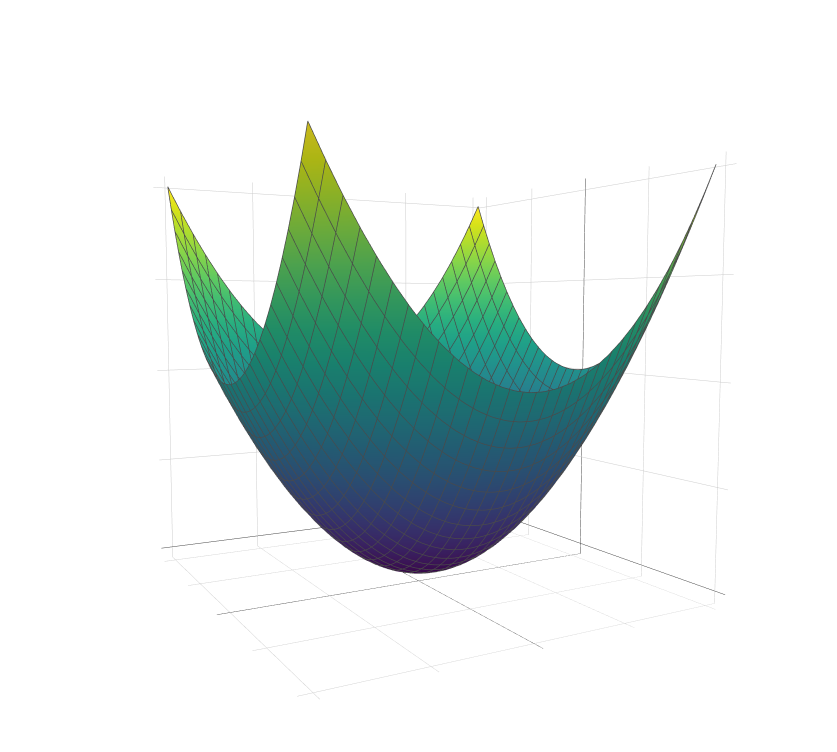
\includegraphics[width=.8\linewidth]{Screenshot (30)}
  \captionof{figure}{Proper paraboloid}
  \label{fig:test1}
\end{subfigure}%
\begin{subfigure}{.5\textwidth}
  \centering
  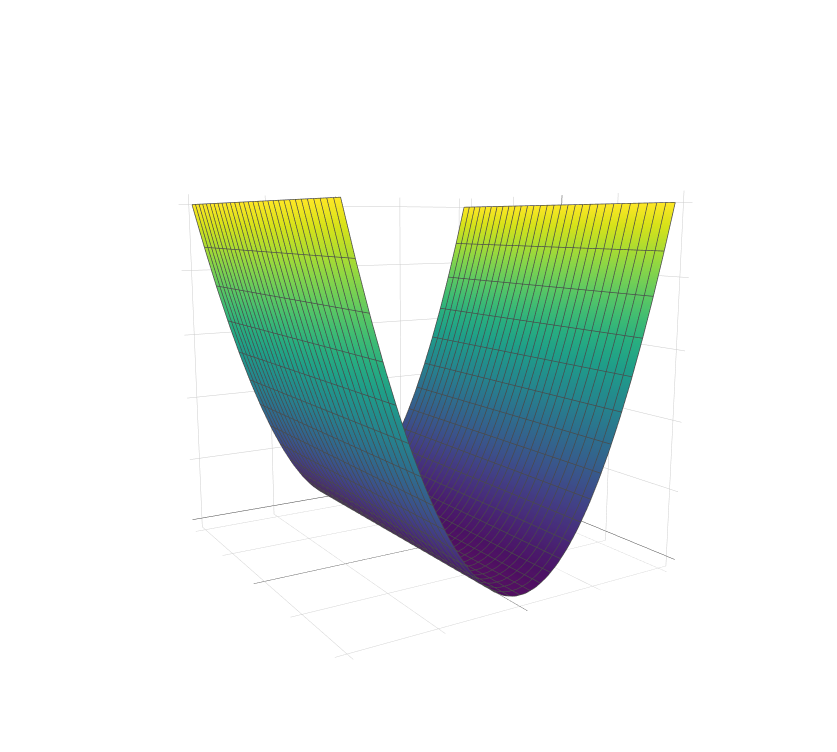
\includegraphics[width=.8\linewidth]{Screenshot (31)}
  \captionof{figure}{Degenerate paraboloid}
  \label{fig:test2}
\end{subfigure}
\end{figure}


\begin{align*}
\frac{d^{2}}{d\theta ^{2}} J_{N}(\theta) & =\frac{2}{N}\sum _{i=1}^{N} \varphi (i) \varphi (i)\transpose \ \text{nonsingular} \ \text{(pos. def.)} & \Longrightarrow \ & \text{proper paraboloid (unique min.)}\\
\frac{d^{2}}{d\theta ^{2}} J_{N}(\theta) & =\frac{2}{N}\sum _{i=1}^{N} \varphi (i) \varphi (i)\transpose\text{ singular} & \ \Longrightarrow \ & \text{degenerate paraboloid}
\end{align*}

